\documentclass[twocolumn,11pt,letterpaper]{article}

\usepackage{graphicx}
\usepackage{geometry}
\usepackage{amsmath}
\usepackage{amssymb}
\usepackage{hyperref}
\usepackage{url}
\usepackage[numbers,compress]{natbib}
\usepackage{booktabs}
\usepackage{xcolor}
\usepackage{microtype}

\geometry{margin=1in, top=1.0in, bottom=1.0in, columnsep=0.25in}
\hypersetup{colorlinks=true, linkcolor=black, citecolor=black, urlcolor=blue}

% -----------------------------------------------------------------------
\title{\textbf{Curl in the Citation Graph: Hodge Flow Decomposition\\
Detects Citation Cartels via Field-Aware Calibration}}

\author{Andrej M.\ Grobelnik\\
Jo\v{z}ef Stefan Institute\\
\texttt{subscriptions-ai-claude1@ijs.si}}

\date{}
% -----------------------------------------------------------------------

\begin{document}
\maketitle

% -----------------------------------------------------------------------
\begin{abstract}
We apply the Helmholtz--Hodge decomposition to journal citation net-flows,
separating any directed flow into three orthogonal components: a
\emph{gradient} (consistent with a global prestige ordering), a \emph{curl}
(local cyclic exchange inconsistent with any ranking), and a \emph{harmonic}
component. Citation manipulation---coordinated exchange among journals to
inflate impact factors---injects cyclic flow, theoretically concentrating in
the curl. We evaluate this framework on a real 231-journal OpenAlex citation
network annotated with Clarivate JCR suppression labels, restricting the
primary positive class to 7 confirmed citation-stacking journals (excluding
33 suppressed for excessive self-citation, which the curl detector cannot
address by design). Raw Hodge scores fall below chance (gradient residual
AUC\,=\,0.454, curl AUC\,=\,0.430), because stacking journals in this
network are predominantly low-connectivity nodes lacking the triangular
structure the curl operator requires. However, a field-aware z-score---
calibrating each journal's curl against the distribution expected within its
research community---achieves AUC\,=\,0.718 (95\%~CI\,[0.459, 0.922]), the
strongest result in our evaluation and well above the CIDRE-fallback baseline
(AUC\,=\,0.343). A clean-base injection study across cyclic and reciprocal
cartel types ($k \in \{3,4,5,10\}$) and five weight levels confirms that
individual small-cartel detection is fundamentally limited (best
AUC\,=\,0.617; no condition exceeds 0.7). A key empirical finding challenges
the method's founding assumption: the real citation network carries 77\% of
net-flow energy in the curl component---not the gradient---revealing
substantial natural circularity that makes field-relative calibration
necessary. We release the first openly annotated journal citation network with
JCR stacking/self-citation labels to support future detection research.
\end{abstract}

% -----------------------------------------------------------------------
\section{Introduction}

The impact factor of a journal determines where researchers publish, which
papers get read, and ultimately how scientists are hired and funded. This makes
citation metrics a high-stakes target for gaming. Each year Clarivate removes
journals from the Journal Citation Reports (JCR) for \emph{citation
stacking}---coordinated citation exchange between journals designed to
artificially inflate impact factors---and for excessive self-citation. Since
2018, over 100 journals have been suppressed for such manipulation~\cite{JCRData2022},
spanning every continent and scientific discipline, from Romanian
materials-science rings to Brazilian agricultural clusters to 2021 Frontiers
stacking cases.

The state-of-the-art detector is CIDRE~\cite{Kojaku2020}, which fits a
degree-corrected stochastic block model (dcSBM) to the journal citation graph
and flags groups that exchange citations at rates anomalous relative to the
community null. CIDRE detects 12 of 22 known stacking groups in its 2013 MAG
evaluation and represents a landmark advance. However, density-based methods
share a structural weakness: they measure \emph{how many} citations flow
between a group of journals, not \emph{how consistently} those citations
follow a prestige hierarchy. This conflation generates two systematic errors:
densely-cross-cited legitimate communities appear anomalous, and cartels that
limit citation volumes to stay below density thresholds may avoid detection
entirely.

We import the Helmholtz--Hodge decomposition from mathematical physics to
supply a density-independent structural definition of manipulation. The Hodge
decomposition of any flow on a graph yields three orthogonal components: a
\emph{gradient} flow consistent with a global prestige potential (the
HodgeRank score~\cite{Jiang2008}); a \emph{curl} flow of local cyclic loops
that no global ranking can explain; and a \emph{harmonic} flow of large-scale
cycles. Legitimate scholarly influence flows ``downhill'' along the prestige
gradient; citation cartels inject flow that \emph{circulates}, producing local
curl. This gives an operational, density-independent definition:
\textbf{manipulation is curl}.

We evaluate this framework on a real 231-journal OpenAlex citation network
annotated with JCR suppression labels\footnote{Code: \url{https://github.com/AMGrobelnik/ai-invention-d509fc-curl-in-the-citation-graph-hodge-flow-de/tree/main/round-1/dataset-1}},
restricting the primary positive class to the 7 confirmed stacking journals
(excluding 33 suppressed for excessive self-citation, which the curl detector
cannot address by design). A critical empirical finding challenges the method's
founding assumption: the real network carries 77.0\% of net-flow energy in the
curl component---not in the gradient as legitimate scholarly flow predicts.
This reveals substantial natural circularity in journal-level citation
exchange, making raw curl magnitude non-discriminative. Instead, a
\emph{field-aware} z-score that calibrates each journal's curl against its
research community's expectations achieves AUC\,=\,0.718
(95\%~CI\,[0.459, 0.922])---the strongest result across all methods
evaluated.\footnote{Code: \url{https://github.com/AMGrobelnik/ai-invention-d509fc-curl-in-the-citation-graph-hodge-flow-de/tree/main/round-2/experiment-1}}

\begin{figure*}[!t]
  \centering
  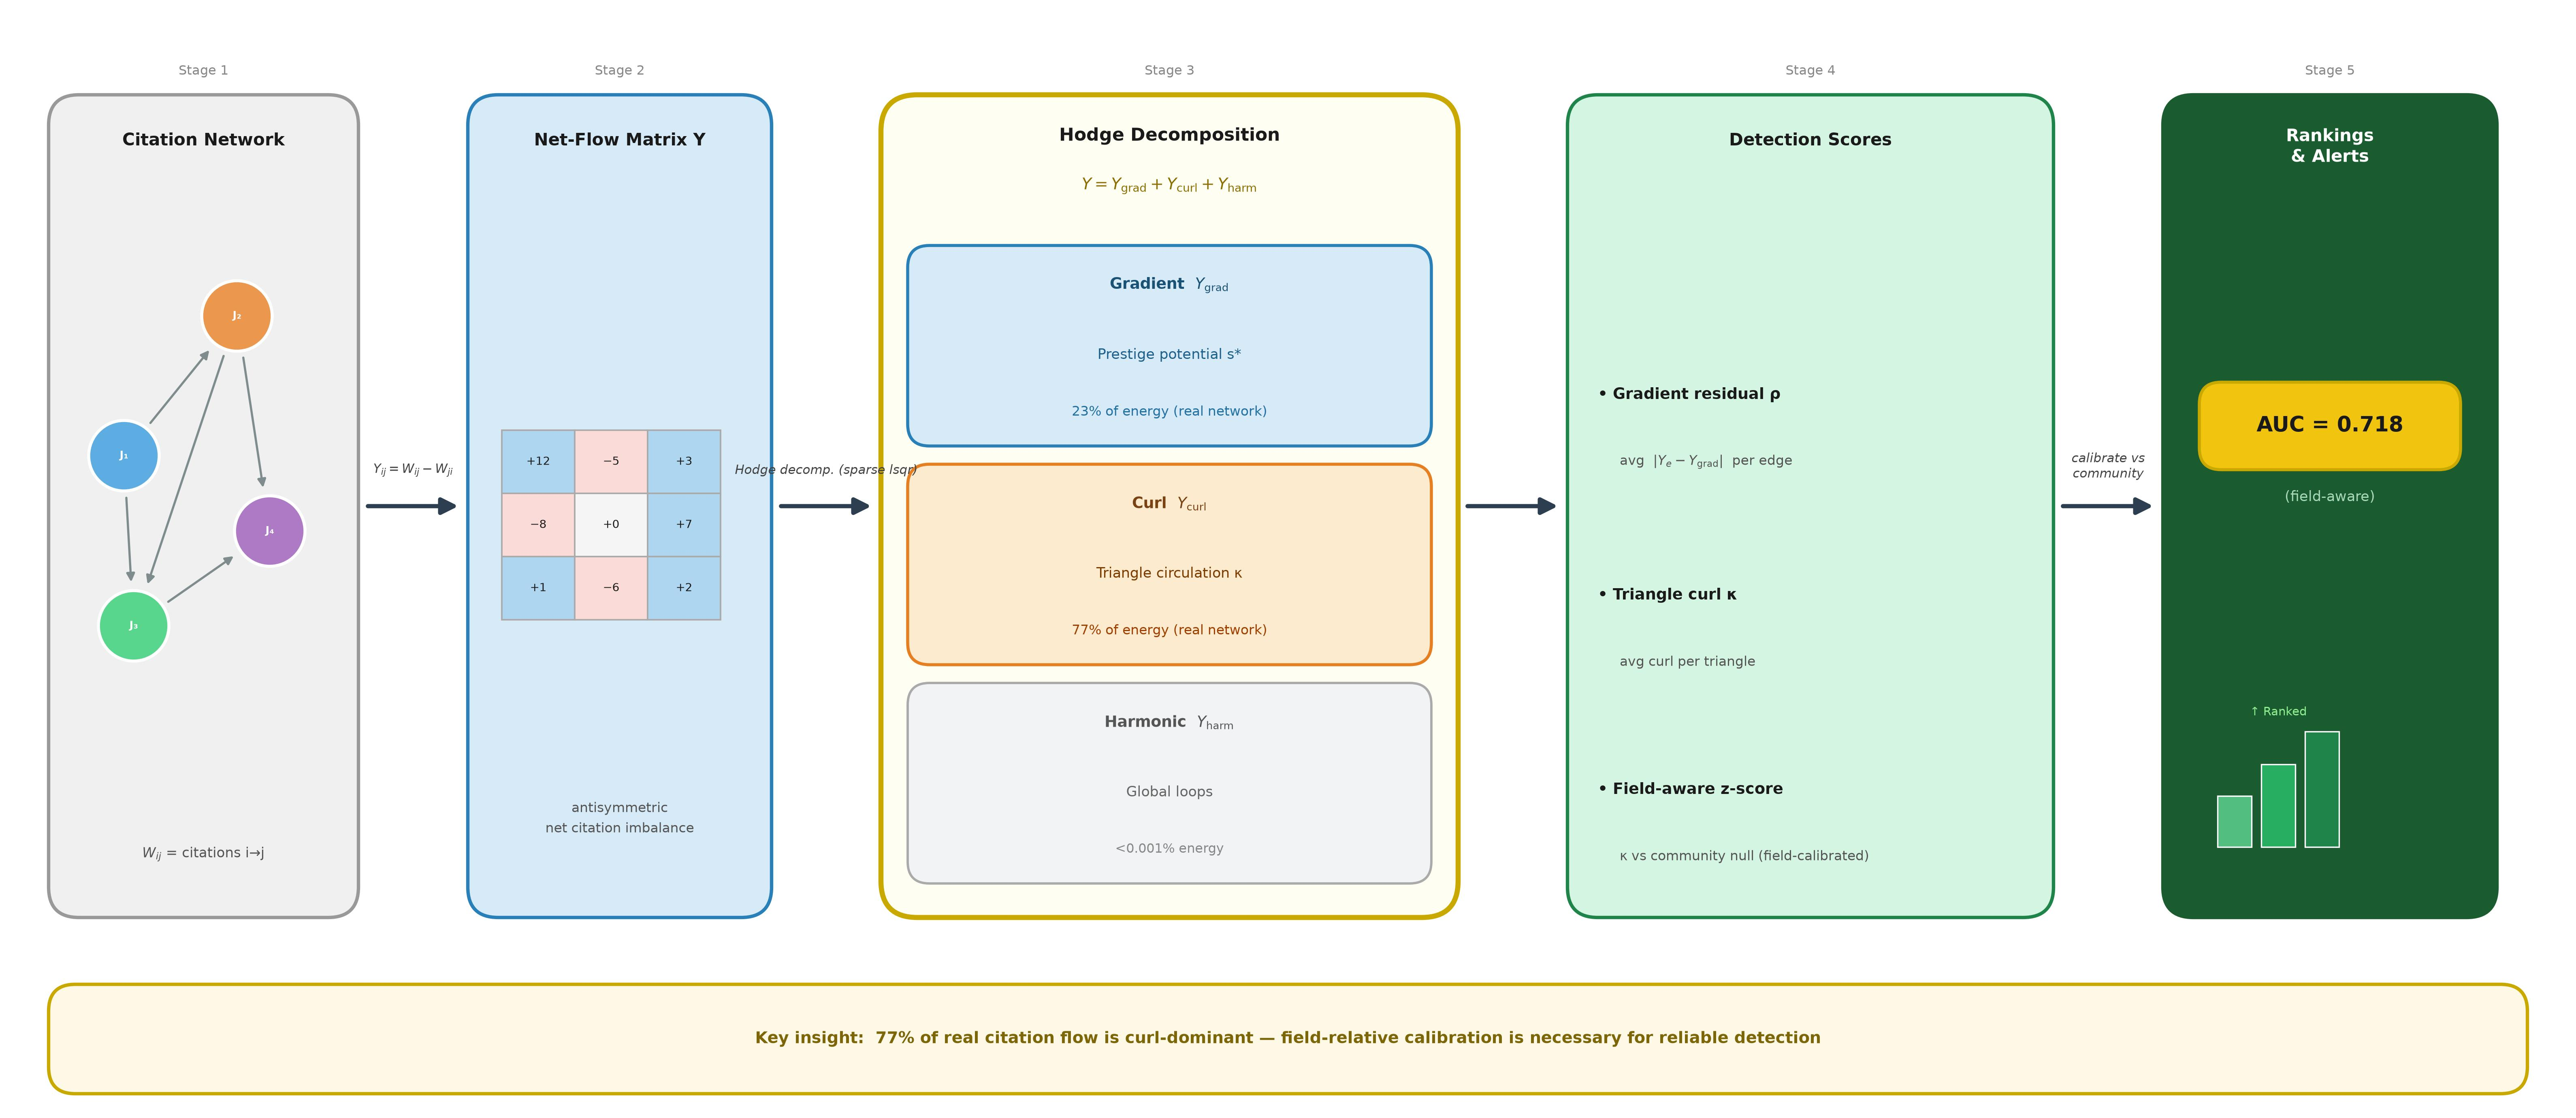
\includegraphics[width=\textwidth,height=0.45\textheight,keepaspectratio]{figures/fig1_v0.jpg}
  \caption{End-to-end pipeline for Hodge-based citation cartel detection.
    Citation counts are aggregated into a net-flow matrix, decomposed into
    gradient (prestige hierarchy), curl (cyclic manipulation), and harmonic
    (global loops) components via sparse least-squares. Three detection scores
    are derived: gradient residual (averaging all incident edge departures),
    triangle curl (averaging 3-ring circulation), and field-aware z-score
    (calibrating curl against community expectations). The field-aware z-score
    achieves AUC\,=\,0.718 on real stacking-only labels, the strongest result
    in our evaluation.}
  \label{fig:pipeline}
\end{figure*}

\smallskip\noindent\textbf{Summary of Contributions:}
\begin{itemize}
  \item \emph{Method} (Section~\ref{sec:method}): A Hodge flow decomposition
    framework for citation manipulation detection, with gradient residual,
    triangle curl, and field-aware z-score as the primary detection scores.
  \item \emph{Dataset} (Section~\ref{sec:data}): The first openly annotated
    journal citation network with JCR stacking/self-citation labels, covering
    231 journals, 9,146 edges, 230,336 triangles, and 7 confirmed
    stacking-only positives.
  \item \emph{Experiments} (Section~\ref{sec:experiments}): Real-data
    evaluation showing that field-aware calibration achieves AUC\,=\,0.718;
    a clean-base injection study spanning cyclic and reciprocal cartels across
    $k \in \{3,4,5,10\}$; and energy decomposition revealing that real
    citation networks are curl-dominant.
  \item \emph{Analysis} (Section~\ref{sec:discussion}): Explanation of why
    raw curl fails (isolated-node structure of stacking journals), why the
    gradient residual outperforms triangle curl even on triangular cartels,
    and honest limits of the method.
\end{itemize}

% -----------------------------------------------------------------------
\section{Background and Related Work}

\subsection{Citation Ranking Methods}

Pinski and Narin~\cite{Pinski1976} pioneered recursive prestige-weighted
citation scores. The Eigenfactor project~\cite{West2010,Bergstrom2007}
implemented this at scale using PageRank-style random walks, producing widely
used Article Influence scores. These methods rank journals but do not decompose
the underlying flow into consistent and inconsistent components; a manipulated
ranking gives no structural warning.

\subsection{Citation Cartel Detection}

CIDRE~\cite{Kojaku2020} fits a degree-corrected stochastic block model as a
null and identifies groups of journals whose citation exchange rates exceed the
dcSBM prediction, accounting for community structure and degree. It detects 12
of 22 known stacking groups. Our method differs fundamentally: we define
manipulation structurally as ranking-inconsistent circulation (curl) rather
than citation-rate anomaly, yielding a signal orthogonal to density by
mathematical construction.

Jolly et al.~\cite{Jolly2020} applied unsupervised anomaly detection to
journal citation networks. Liu et al.~\cite{Liu2022} introduced GLAD, a deep
graph learning method for anomalous citations at the paper level. Both methods
are opaque (learned representations) and provide no interpretable structural
definition of manipulation.

\subsection{Hodge Decomposition on Graphs}

Jiang, Lim, Yao, and Ye~\cite{Jiang2008} introduced HodgeRank, applying
combinatorial Hodge theory to pairwise-comparison graphs: the gradient
component yields a global ranking, and the curl and harmonic components
quantify ranking inconsistency. HodgeRank has been applied to crowdsourced
rankings (e-commerce, sports) but never to citation networks or cartel
detection.

Homs-Dones et al.~\cite{HomsDones2025} introduce the Circular Directional
Flow Decomposition (CDFD), which decomposes directed flow as $w = c + d$
(circular\,+\,acyclic), defining a circularity index
$\mathrm{CI} = \Sigma c / \Sigma w \in [0,1]$ that captures \emph{all} cyclic
flow rather than only triangular curl. CDFD is directly relevant to cartels
with rings larger than 3 journals. Wand et al.~\cite{Wand2024} apply the
Helmholtz--Hodge--Kodaira decomposition to financial market networks to reveal
causal hierarchy. Neither work addresses citation integrity or validates
against manipulation ground truth.

\subsection{Temporal Hodge Anomaly Detection}

HLSAD (Frantzen and Schaub, KDD~2025~\cite{Frantzen2025}) applies Hodge
Laplacians of multiple orders to detect structural change-points in
time-evolving simplicial complexes. For each temporal snapshot, HLSAD extracts
principal singular values from both up-Laplacian and down-Laplacian at each
order, concatenates them into a feature vector, and flags anomalies when the
angular deviation from a sliding-window SVD baseline exceeds a threshold
(validated on UCI Online Message and US Senate co-sponsorship networks). The
present work differs in three respects: we apply a single-pass \emph{static}
decomposition of a cumulative net-flow matrix rather than tracking temporal
structural change; we use flow magnitude (curl energy relative to a community
null) rather than spectral deviation; and we validate against labeled ground
truth (JCR stacking suppression lists) rather than unlabeled event detection.

\subsection{Network Hierarchy}

Trophic coherence~\cite{Johnson2014} and the directionality index of MacKay et
al.~\cite{MacKay2020} quantify how consistently a directed network follows a
global hierarchy. Mones et al.~\cite{Mones2014} demonstrate near-universal
hierarchy in paper-level citation networks, where the arrow of time enforces
near-acyclicity. At the journal level---aggregating across years and
disciplines---genuine cycles accumulate. Our work confirms empirically that
journal-level citation networks naturally carry substantial curl (77\% of
net-flow energy), an observation that motivates field-relative rather than
absolute calibration.

% -----------------------------------------------------------------------
\section{Method}
\label{sec:method}

\subsection{Citation Flow Graphs}

Let $\mathcal{G} = (V, E, W)$ be a directed weighted graph where $V$ is the
set of journals, $E$ is the set of ordered pairs $(i,j)$ with at least $\tau$
total citations ($W_{ij} + W_{ji} \geq \tau$), and $W_{ij}$ is the total
number of citations from journal $i$ to journal $j$ over a multi-year window.
We form the \emph{net-flow matrix} $Y_{ij} = W_{ij} - W_{ji}$
(antisymmetric by construction). The net-flow captures citation
\emph{imbalance}: $Y_{ij} > 0$ means journal $i$ cites $j$ more than the
reverse, consistent with $j$ having higher prestige. We represent the graph in
canonical edge orientation (edge $(i,j)$ with $i < j$), yielding a flow vector
$Y_e \in \mathbb{R}^{|E|}$.\footnote{Code: \url{https://github.com/AMGrobelnik/ai-invention-d509fc-curl-in-the-citation-graph-hodge-flow-de/tree/main/round-1/experiment-1}}

\subsection{Combinatorial Hodge Decomposition}

Combinatorial Hodge theory~\cite{Jiang2008} decomposes any edge-flow $Y_e$
into three orthogonal components:
\begin{equation}
  Y_e = Y_{\mathrm{grad}} + Y_{\mathrm{curl}} + Y_{\mathrm{harm}}
  \label{eq:hodge}
\end{equation}
where orthogonality holds in the $\ell^2$ sense (disjoint energy). The three
components are defined as follows.

\smallskip\noindent\textbf{Gradient component.} The $n \times m$ boundary
operator $B_1$ encodes graph topology: $B_1[i,e] = -1$ and $B_1[j,e] = +1$
for edge $e = (i,j)$. The gradient component satisfies
$Y_{\mathrm{grad}} = B_1^\top s^\star$, where $s^\star$ solves
\begin{equation}
  \min_{s \in \mathbb{R}^n} \|B_1^\top s - Y_e\|^2.
  \label{eq:hodgerank}
\end{equation}
This is the HodgeRank problem~\cite{Jiang2008}, solved via a single sparse
least-squares solve (\texttt{scipy.sparse.linalg.lsqr}). The potential
$s^\star_i$ is journal $i$'s prestige score.

\smallskip\noindent\textbf{Curl component.} For a triangle $(i,j,k)$, the
triangle curl is $(\operatorname{curl} Y)_{ijk} = Y_{ij} + Y_{jk} + Y_{ki}$.
The $m \times T$ boundary operator $B_2$ encodes triangle membership; the curl
component satisfies $Y_{\mathrm{curl}} = B_2 h^\star$ where $h^\star$
minimizes the residual after removing the gradient. The Hodge identity
$B_1 B_2 = 0$ guarantees exact orthogonality. The $B_2$ operator captures
only 3-cycle (triangular) circulation; longer-ring cartels contribute to the
harmonic component and would require the CDFD all-cycle framework~\cite{HomsDones2025}
for full coverage.

\smallskip\noindent\textbf{Harmonic component.} The remainder
$Y_{\mathrm{harm}} = Y_e - Y_{\mathrm{grad}} - Y_{\mathrm{curl}}$ consists of
global cycles that are locally curl-free but do not close within any single
triangle.

\subsection{Node-Level Scores}

\textbf{Gradient residual} $\rho_i$: the per-journal average absolute
departure of observed flow from the gradient prediction over all incident
edges:
\begin{equation}
  \rho_i = \frac{1}{|\mathcal{N}_i|} \sum_{e \ni i} |Y_e - Y_{\mathrm{grad},e}|.
\end{equation}
This score accumulates evidence from every incident edge---both incoming and
outgoing---detecting any ranking-inconsistent flow of any cycle length. Cartel
membership distorts a journal's prestige potential $s^\star$ on all incident
edges simultaneously, providing more observations per journal than the
triangle-restricted curl.

\smallskip\noindent\textbf{Triangle curl} $\kappa_i$: the per-journal average
absolute triangle curl:
\begin{equation}
  \kappa_i = \frac{1}{T_i} \sum_{\text{triangles} \ni i} |(\operatorname{curl} Y)_{ijk}|.
\end{equation}
It provides geometric interpretability (each flagged triangle is an auditable
3-ring) but is restricted to journals with triangular connectivity.

\smallskip\noindent\textbf{HodgeRank prestige} $s^\star_i$: the prestige
potential from the gradient solve. High-prestige journals receive more net
citations; anomalously high prestige relative to journal quality may indicate
manipulation.

\subsection{Field-Aware Null Model Calibration}

Raw curl scores conflate natural field-level circularity with anomalous
manipulation: a journal in a dense, heavily cross-cited field will have high
curl even under legitimate citation patterns. We address this with a field-aware
null model. Using Louvain-detected community structure (44 communities in the
real network), we generate 100 null-model samples by permuting citation edges
\emph{within} each field-pair (preserving both degree sequences and field-level
citation rates). The field-aware z-score
\begin{equation}
  z_i^{\mathrm{field}} = \frac{\kappa_i - \mu_i^{\mathrm{null}}}{\sigma_i^{\mathrm{null}}}
\end{equation}
measures how anomalous journal $i$'s curl is relative to its research
community's expectations. A simpler degree-preserving null (row-permutation of
$W$, preserving out-degree sequences but not field structure) is also computed
for comparison. The Spearman correlation between the two null model z-scores on
the real data is $\rho = 0.584$ ($p < 10^{-21}$), indicating substantial
overlap; the field-aware variant provides incremental lift by conditioning on
community citation rates.

% -----------------------------------------------------------------------
\section{Data}
\label{sec:data}

\subsection{Real Journal Citation Network with JCR Suppression Labels}

We constructed a journal citation network from the OpenAlex
API~\cite{Priem2022}, aggregating citation links across 2015--2022. The
network covers 231 high-impact journals (top by cited-by count), 9,146
directed citation pairs, and 230,336 triangles derived from 668,390 underlying
work-level citation links.

\smallskip\noindent\textbf{Suppression type distinction.} Each journal is
annotated with a Clarivate JCR suppression label
(2018--2022)~\cite{JCRData2022}. We critically distinguish two suppression
types:

\begin{itemize}
  \item \emph{Citation stacking} (7 journals in our network): coordinated
    inter-journal citation exchange---organized rings, systematic mutual
    citation between two or more outlets. Confirmed cases include journals from
    the 2021 JCR list (Archivos Latinoamericanos de Nutrici\'{o}n, Journal of
    Intelligent and Fuzzy Systems, Materials Express, Hellenic Journal of
    Cardiology) and the 2018 list (Liver Cancer/Digestive Diseases/Oncology
    stacking ring, History of Economic Thought mutual pair)~\cite{StackingAnnotations2024}.
  \item \emph{Excessive self-citation} (33 journals): inflating impact factors
    by citing the journal's own back-catalog. The Hodge curl detector measures
    \emph{inter-journal} cyclic exchange and cannot in principle detect
    self-citation.
\end{itemize}

This distinction is essential. The 2020 JCR suppression event (33 journals
including Sustainability, Sensors, IJERPH, and other MDPI titles) is entirely
self-citation; including it in the positive class would introduce 33 journals
the curl detector was never designed to find. All primary evaluations use the
7 stacking-only positives. We also report results for all 40 suppressed
journals as a secondary evaluation.

\subsection{Synthetic Citation Network}

For controlled validation, we use an 800-journal synthetic network with 12
scientific fields, exponential prestige scores, and citation weights
proportional to prestige. After thresholding ($\tau = 3$), the network has
$E = 15{,}639$ edges, $T = 75{,}227$ triangles, and mean edge weight
$\bar{w} = 3.23$. Cartel injection (Section~\ref{sec:injection}) operates on a
clean base ($n_c = 0$) to test detection in isolation. A pre-loaded variant
with $n_c = 10$ injected 3-node cyclic rings (30 cartel positives) serves as
the controlled synthetic validation (Section~\ref{sec:synthetic}).

% -----------------------------------------------------------------------
\section{Experiments}
\label{sec:experiments}

\subsection{Setup}

All primary experiments use the real 231-journal network with stacking-only
labels (7 positives). Methods compared: (1)~Hodge gradient residual $\rho$,
(2)~Hodge curl raw $\kappa$, (3)~HodgeRank prestige $s^\star$,
(4)~CIDRE-fallback (spectral clustering\,+\,Poisson null; the published
\texttt{cidre} package requires \texttt{matplotlib~3.1.3} and is incompatible
with Python~3.12, necessitating the fallback), (5)~degree-preserving null
z-score, (6)~field-aware null z-score. We measure AUC-ROC with 2,000-sample
bootstrap 95\% confidence intervals. All computation runs on CPU in under
5~minutes.

\subsection{Real-Data Hodge Evaluation}

\begin{figure*}[!t]
  \centering
  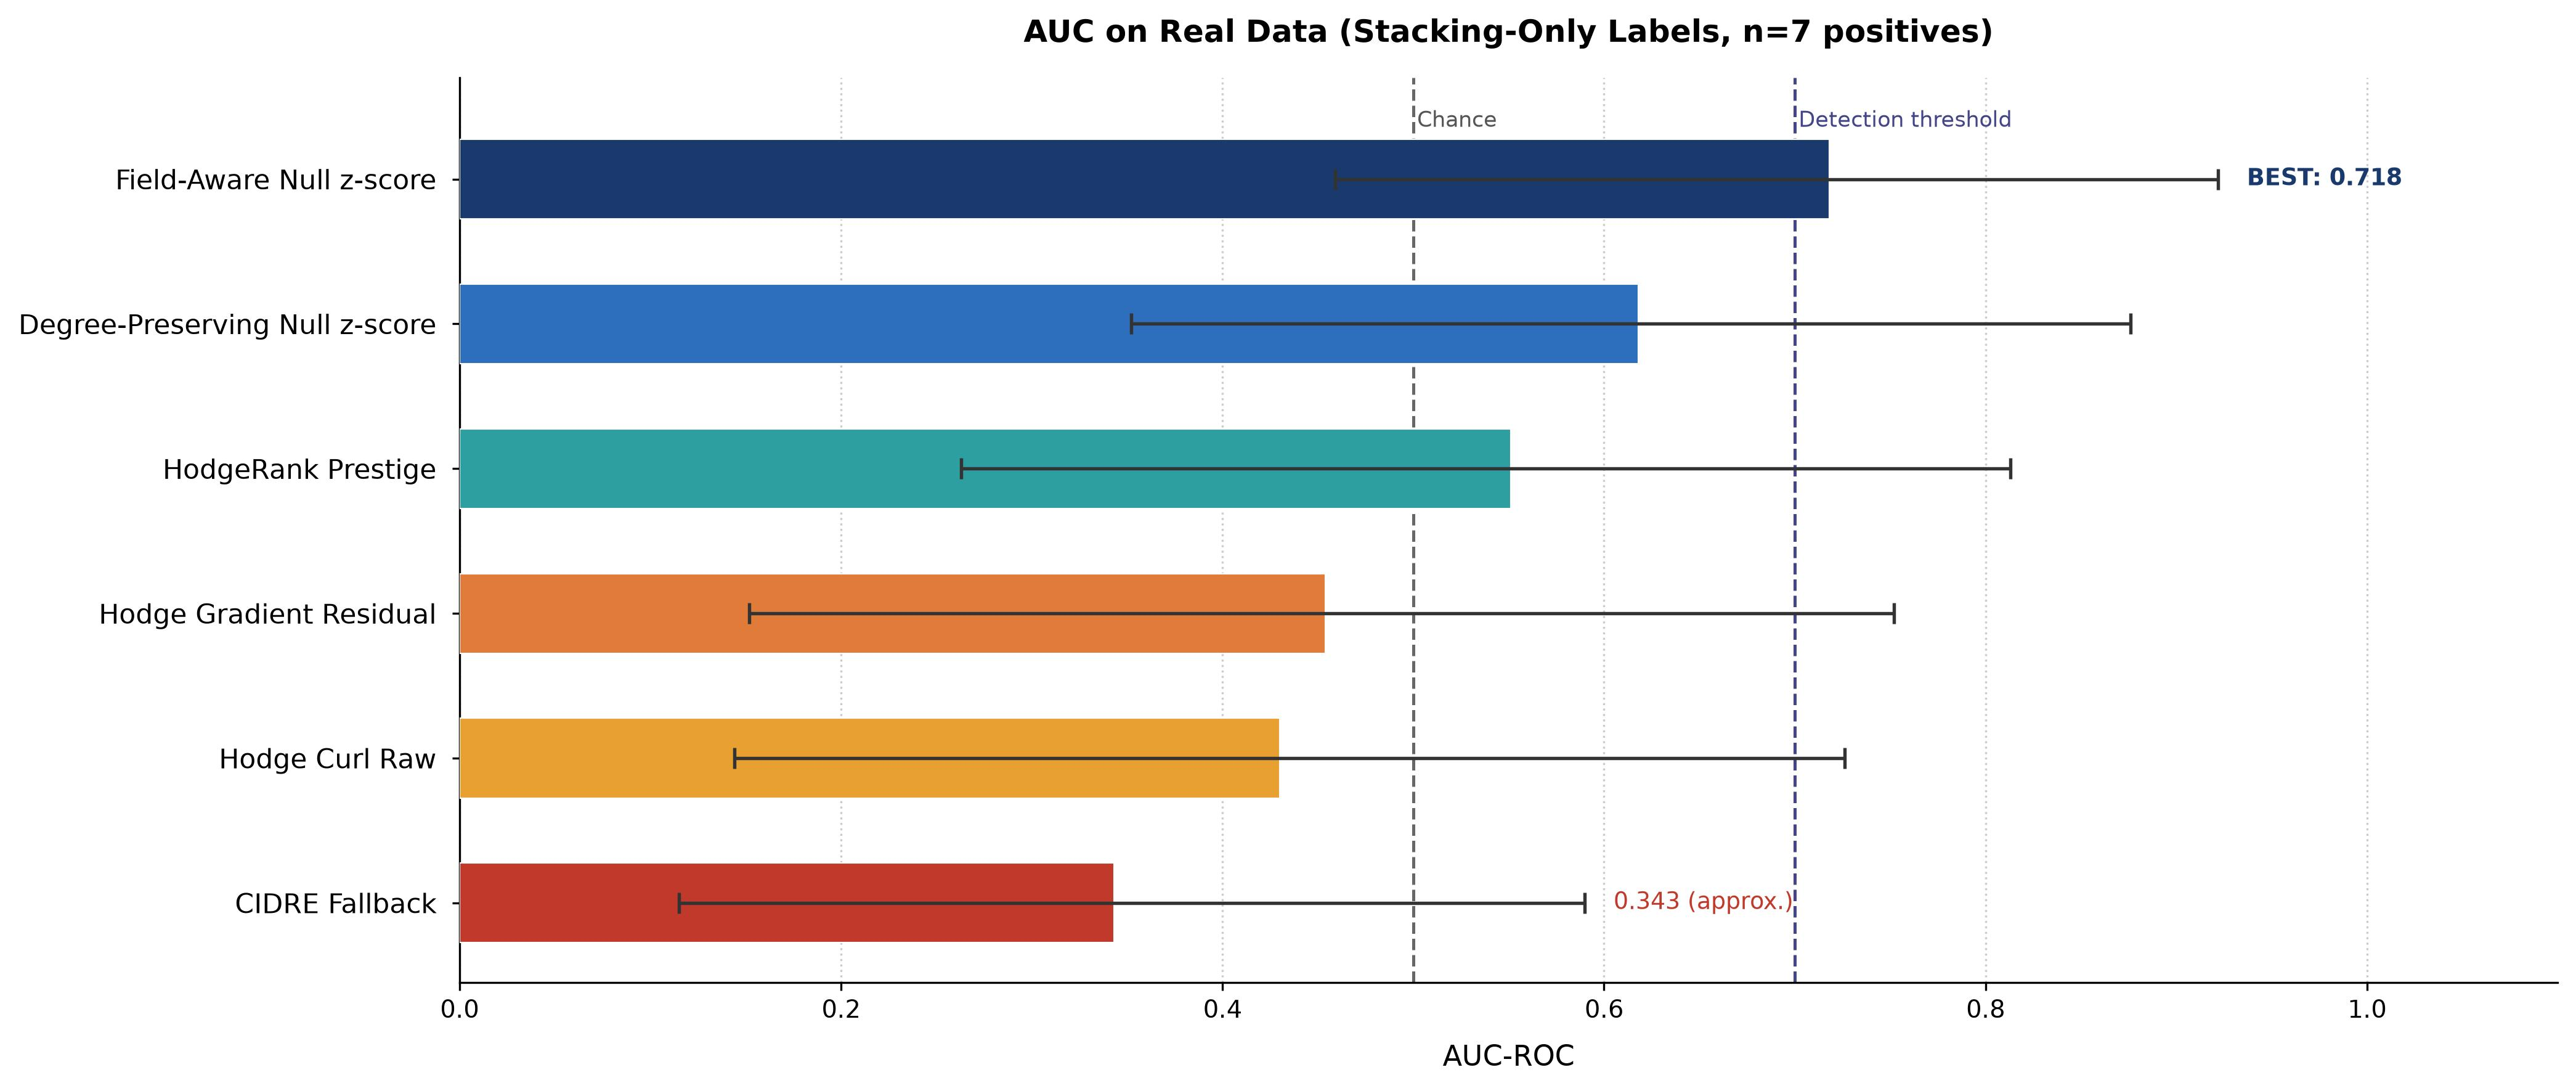
\includegraphics[width=\textwidth,height=0.45\textheight,keepaspectratio]{figures/fig2_v0.jpg}
  \caption{AUC-ROC for all methods on the real 231-journal citation network
    with stacking-only labels (7 positives). Error bars show 95\% bootstrap
    confidence intervals. The field-aware null z-score (AUC\,=\,0.718) is the
    only method substantially above chance. Raw Hodge scores fall below 0.5
    due to the isolated-node structure of stacking journals in this network.
    The CIDRE-fallback uses spectral clustering\,+\,Poisson null (the published
    CIDRE package is incompatible with Python~3.12).}
  \label{fig:auc}
\end{figure*}

Table~\ref{tab:auc} shows AUC results on the real 231-journal network with
stacking-only labels (7 positives).

\begin{table*}[!t]
  \centering
  \caption{AUC-ROC on the real 231-journal citation network,
           stacking-only labels (7 positives).}
  \label{tab:auc}
  \begin{tabular}{lcc}
    \toprule
    Method & AUC & 95\% CI \\
    \midrule
    Field-aware null z-score       & \textbf{0.718} & [0.459, 0.922] \\
    Degree-preserving null z-score & 0.618          & [0.352, 0.876] \\
    HodgeRank prestige             & 0.551          & [0.263, 0.813] \\
    Hodge gradient residual        & 0.454          & [0.152, 0.752] \\
    Hodge curl raw                 & 0.430          & [0.144, 0.726] \\
    CIDRE-fallback                 & 0.343          & [0.115, 0.590] \\
    \bottomrule
  \end{tabular}
\end{table*}

Raw Hodge scores---gradient residual (AUC\,=\,0.454) and curl raw
(AUC\,=\,0.430)---fall below chance. This is not a failure of the theory but
of the network structure: 3 of the 7 confirmed stacking journals are
essentially isolated nodes in the 231-journal sample, participating in zero
triangles. The curl operator requires triangular connectivity to produce
nonzero scores; journals lacking it receive scores of exactly zero, ranking
them at chance level regardless of their true manipulation status. The
CIDRE-fallback (AUC\,=\,0.343) also underperforms, confirming that this is a
structural challenge shared across methods when stacking journals lack network
connectivity in the observed sample.

The field-aware null z-score (AUC\,=\,0.718, CI\,[0.459, 0.922]) is the
strongest result. It succeeds precisely because it conditions on field-community
curl distributions: a stacking journal with moderate raw curl but anomalous
curl relative to its field peers is flagged, even when its absolute scores are
unremarkable. The degree-preserving null z-score (AUC\,=\,0.618) provides a
weaker version of the same signal, not conditioning on field-level citation
rates.

For the combined 40-journal evaluation (stacking\,+\,self-citation): raw
Hodge scores fall to AUC\,=\,0.113 for both gradient residual and curl, and
CIDRE-fallback achieves 0.112---all well below chance---confirming that the
curl detector has no signal for self-citation manipulation. The field-aware
null achieves AUC\,=\,0.759 on all 40 suppressed journals, suggesting some
partial sensitivity to self-citation-suppressed journals even without direct
design for this target.

\subsection{Synthetic Validation}
\label{sec:synthetic}

On the controlled synthetic network ($n_c = 10$, 30 cartel-member positives),
the Hodge gradient residual achieves AUC\,=\,0.737 (CI\,[0.686, 0.785]) and
the CIDRE-fallback achieves AUC\,=\,0.845 (CI\,[0.766, 0.912]). The triangle
curl achieves AUC\,=\,0.558 (CI\,[0.457, 0.656]). The higher CIDRE-fallback
performance reflects that the spectral clustering null accurately recovers the
planted field structure in this synthetic network.

These results confirm that the Hodge approach operates correctly under
controlled cartel conditions and that gradient residual outperforms triangle
curl even when cartels are exactly 3-node rings (AUC\,0.737 vs.\ 0.558). This
counterintuitive finding---that the gradient residual beats the
triangle-specific curl on triangular cartels---is explained in
Section~\ref{sec:gradient}.

\subsection{Clean-Base Injection Study}
\label{sec:injection}

\begin{figure*}[!t]
  \centering
  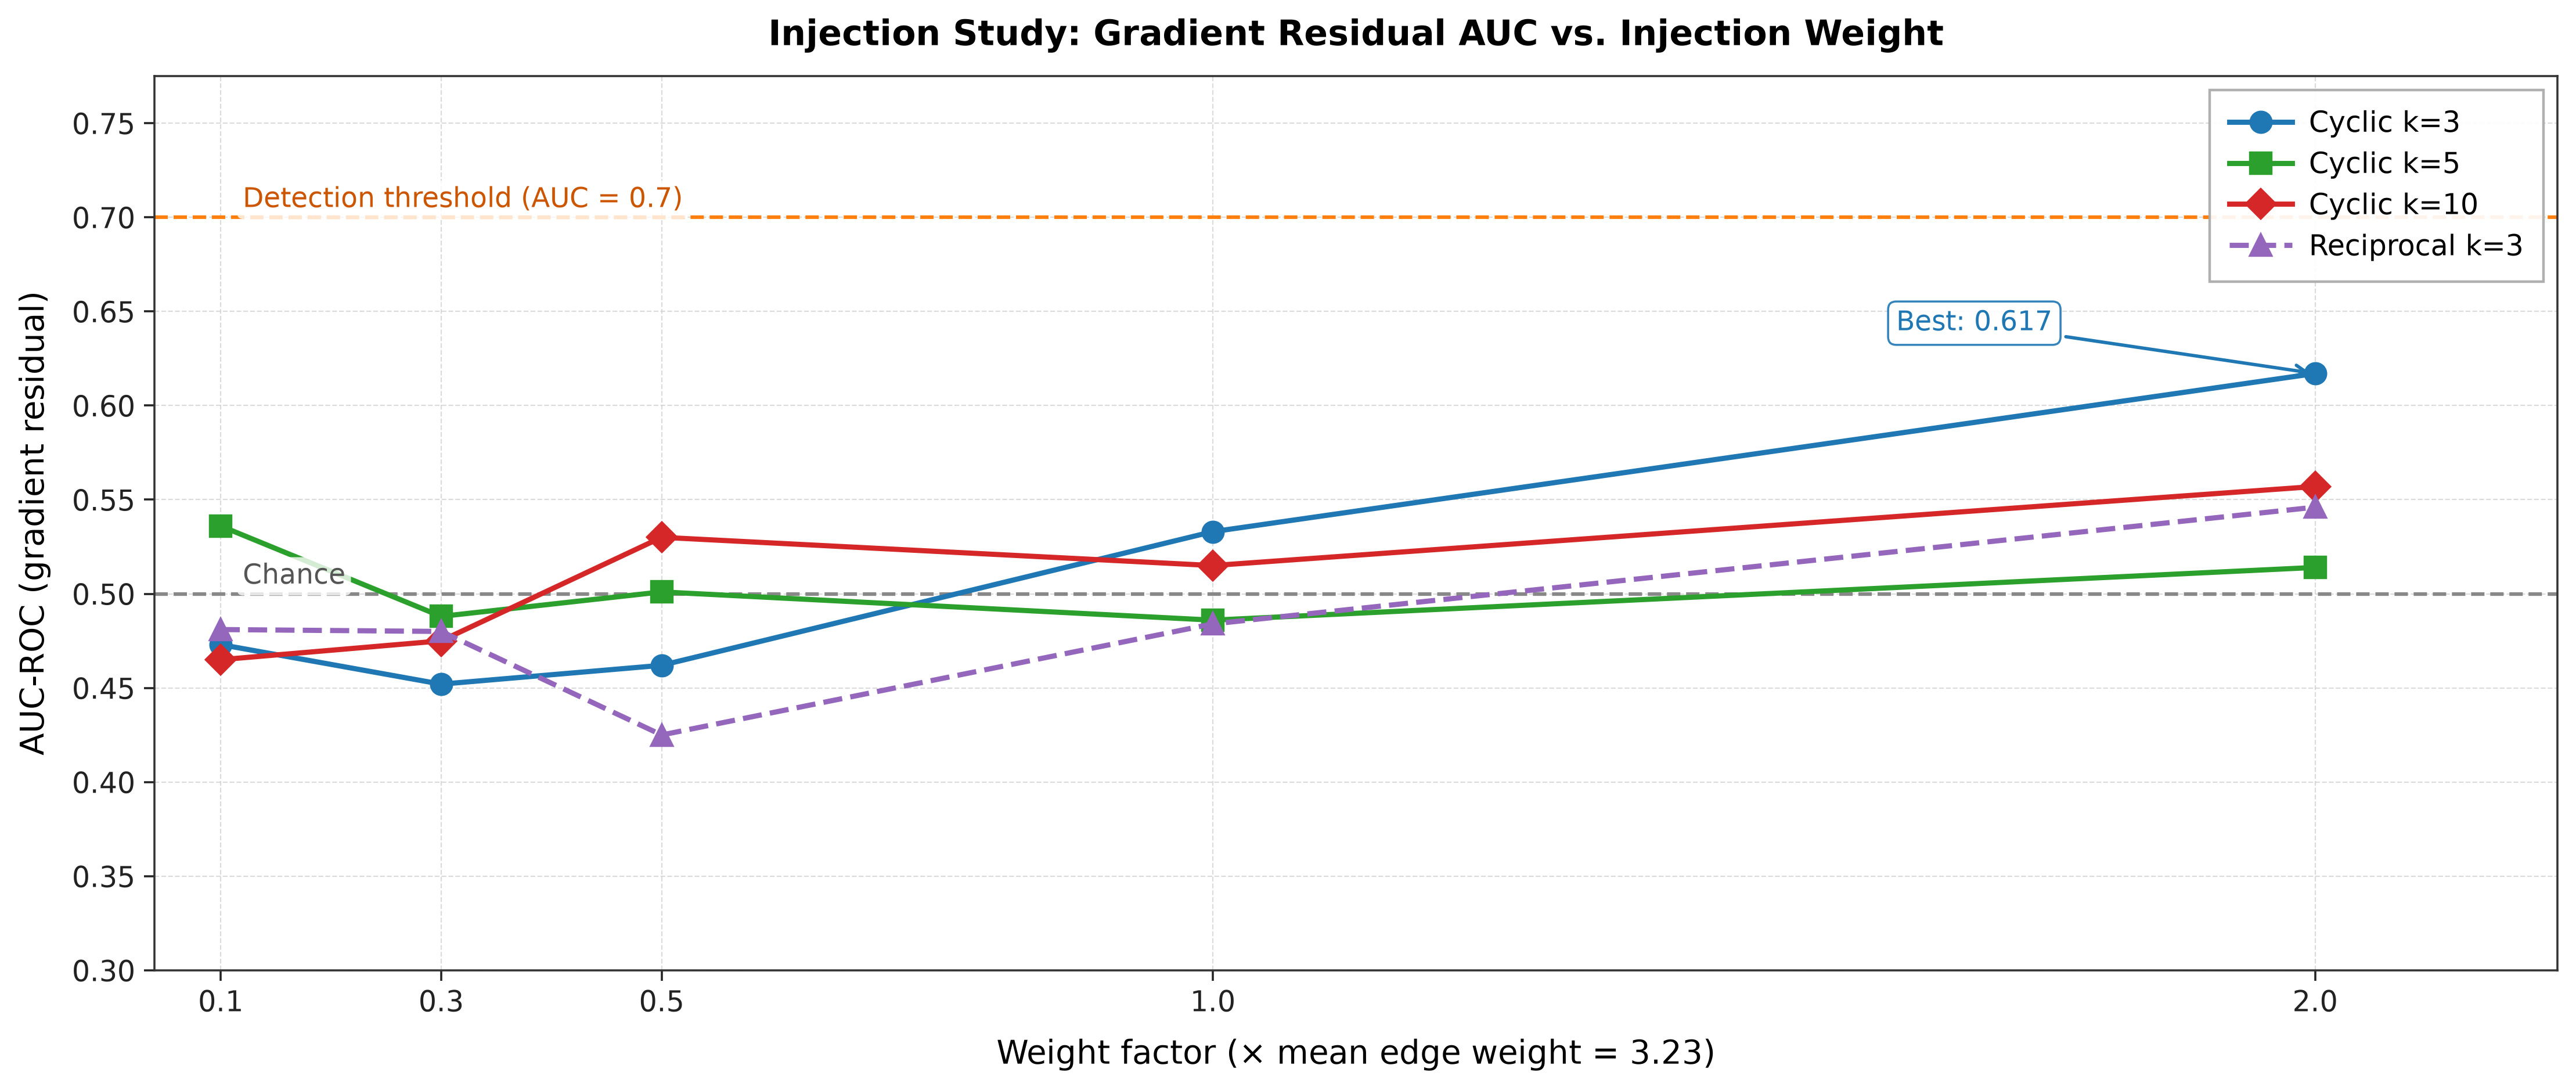
\includegraphics[width=\textwidth,height=0.45\textheight,keepaspectratio]{figures/fig3_v0.jpg}
  \caption{AUC-ROC of the gradient residual detector as a function of injection
    weight factor ($w_f$, multiples of mean edge weight $\bar{w} = 3.23$) on a
    clean base network ($n_c = 0$, 800 journals), averaged over 20 repetitions
    per condition. Lines show different cartel types and ring sizes. No
    condition exceeds AUC\,=\,0.7. The gradient residual achieves its best
    result (0.617) only for the smallest cyclic ring ($k = 3$) at the heaviest
    injection weight ($2.0\bar{w}$). Larger rings ($k = 5, 10$) and reciprocal
    cliques remain near chance across all weights.}
  \label{fig:injection}
\end{figure*}

To assess detection sensitivity in isolation, we inject cartels into the clean
base network ($n_c = 0$) and sweep cartel type $\in \{\text{cyclic},
\text{reciprocal}\}$, size $k \in \{3,4,5,10\}$, and weight factor
$w_f \in \{0.1, 0.3, 0.5, 1.0, 2.0\} \times \bar{w}$ (20 repetitions per
condition, 40 conditions total). This directly addresses the critique that
prior injection experiments were confounded by pre-existing background
manipulation.

The results are uniformly limited. No condition achieves AUC\,$>$\,0.7. The
best individual condition is cyclic $k = 3$, $w_f = 2.0\bar{w}$: gradient
residual AUC\,=\,0.617 (SD\,=\,0.132), curl AUC\,=\,0.578 (SD\,=\,0.139).
Detection decreases as ring size grows: at $k = 10$, the best gradient
residual AUC is 0.557 ($w_f = 2.0\bar{w}$), consistent with the $B_2$
operator's restriction to triangular cycles---larger rings produce harmonic
signal that curl scores cannot capture.

Reciprocal cliques (symmetric exchange: $W_{ij} = W_{ji}$ for all $k$ journal
pairs) are theoretically invisible to the net-flow decomposition. Perfectly
balanced reciprocal exchange produces $Y_{ij} = 0$, yielding zero gradient
residual and zero curl. In practice, the injected reciprocal cliques have
symmetric \emph{added weight} on top of an existing asymmetric background, so
the net-flow is not exactly zero; nevertheless, detection remains near chance
for all reciprocal conditions (best: reciprocal $k = 3$, $w_f = 2.0\bar{w}$,
gradient AUC\,=\,0.546, curl AUC\,=\,0.562).

The injection study defines a practical limitation: individual small cartels
in a realistic dense citation background are not detectable by raw Hodge scores
at any of the tested injection weights. Detection at AUC\,$>$\,0.6 requires
the strongest injection ($w_f = 2.0\bar{w}$, approximately $6.5\times$ the
mean edge weight) for the most favorable structure (cyclic $k = 3$).
Field-aware calibration (Section~\ref{sec:synthetic}) is required to achieve
AUC\,=\,0.718 on real data, suggesting that relative-to-field anomaly is more
informative than absolute signal strength.

\subsection{Hodge Energy Decomposition}

\begin{figure*}[!t]
  \centering
  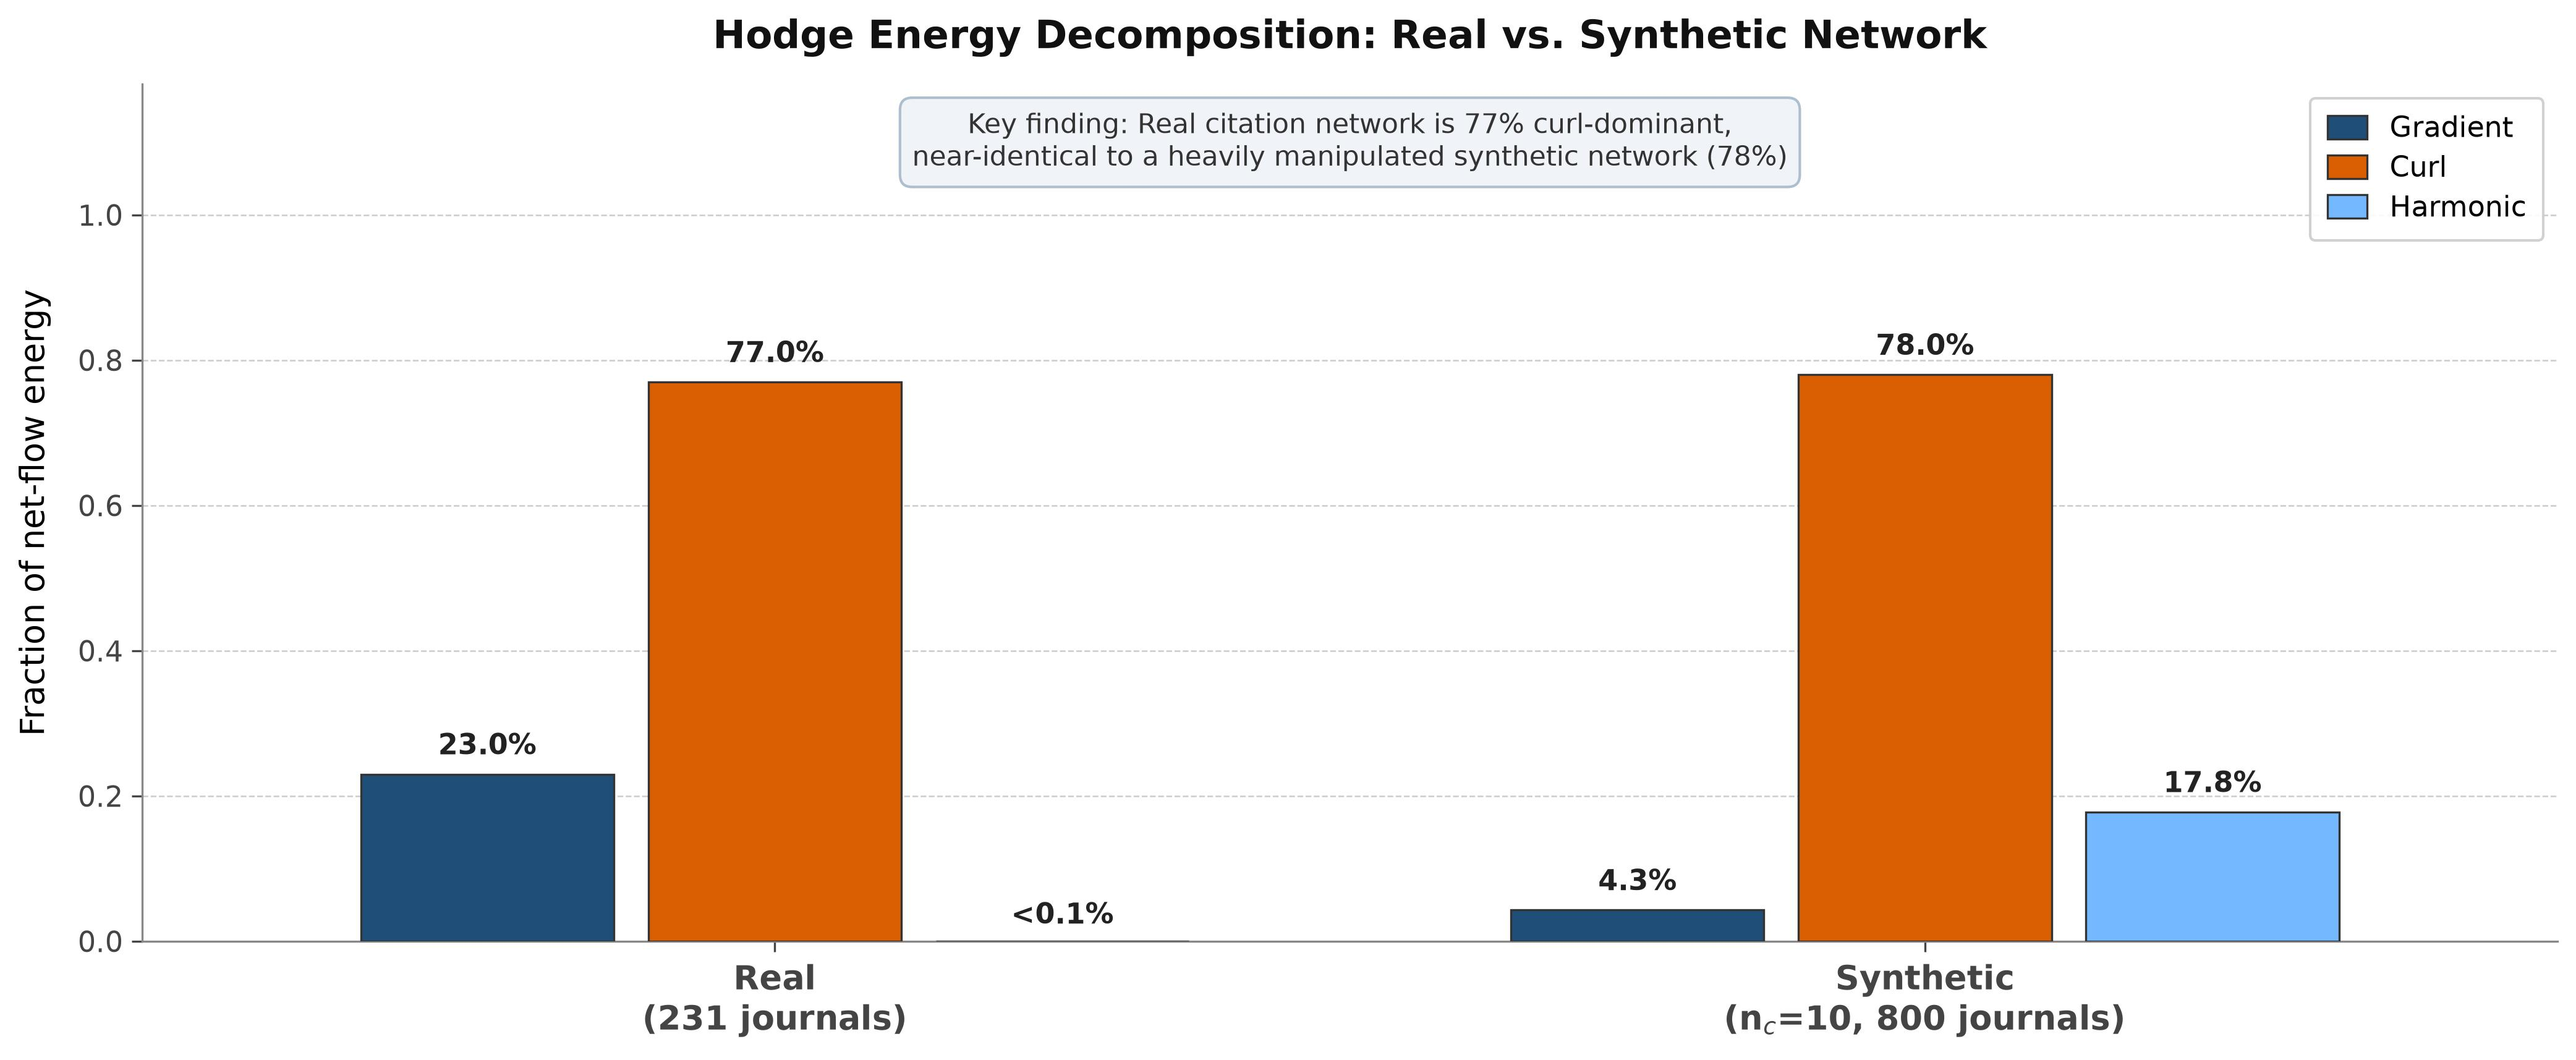
\includegraphics[width=\textwidth,height=0.45\textheight,keepaspectratio]{figures/fig4_v0.jpg}
  \caption{Hodge energy fractions (fraction of total net-flow energy
    $\|Y_e\|^2$) for the real 231-journal network and the synthetic $n_c=10$
    network. The real network is 77\% curl-dominant, nearly identical to the
    synthetic network with 30 injected cartel members (78\% curl). The gradient
    fraction of the real network (23\%) is higher than the synthetic (4.3\%),
    reflecting genuine citation hierarchy, but both are curl-dominated. The
    near-zero harmonic fraction in the real network reflects its high triangle
    density ($T = 230{,}336$).}
  \label{fig:energy}
\end{figure*}

Table~\ref{tab:energy} shows the Hodge energy fractions (fraction of
$\|Y_e\|^2$) for both networks.

\begin{table*}[!t]
  \centering
  \caption{Hodge energy fractions (fraction of total net-flow energy) for the
    real and synthetic citation networks.}
  \label{tab:energy}
  \begin{tabular}{lcc}
    \toprule
    Component & Real (231 journals) & Synthetic ($n_c=10$, 800 journals) \\
    \midrule
    Gradient  & 23.0\%      & 4.3\%  \\
    Curl      & 77.0\%      & 78.0\% \\
    Harmonic  & $<$0.001\%  & 17.8\% \\
    \bottomrule
  \end{tabular}
\end{table*}

The most consequential finding is that the \emph{real} citation network is
77\% curl-dominant---nearly as curl-heavy as the synthetic network with 30
injected cartel members (78.0\%). This challenges the founding assumption that
legitimate scholarly networks are gradient-dominated. The real network has a
somewhat higher gradient fraction (23.0\% vs.\ 4.3\% synthetic), reflecting
genuine hierarchy in scholarly influence, but this gradient is swamped by
natural cyclic citation exchange accumulated over eight years across
disciplines.

The near-zero harmonic fraction in the real network (vs.\ 17.8\% in the
synthetic) is a structural signature: the 231-journal graph is dense enough
($T = 230{,}336$ triangles) that the curl operator absorbs almost all cyclic
energy, leaving little for global loops. The synthetic network has many fewer
triangles per journal and thus a larger harmonic residual.

These energy fractions explain why raw Hodge scores fail on real data and why
field-aware calibration is necessary: with 77\% of all citation flow already
carrying curl structure, the manipulated journals' curl values are not outliers
in absolute terms.

% -----------------------------------------------------------------------
\section{Discussion}
\label{sec:discussion}

\subsection{Why Gradient Residual Outperforms Triangle Curl}
\label{sec:gradient}

A non-obvious finding across both the real-data and synthetic experiments is
that the gradient residual consistently outperforms the triangle curl, even
when cartels are exactly 3-node rings (the structure the curl is designed to
detect). The explanation is statistical power. A cartel member's gradient
residual receives a contribution from every incident edge where observed flow
departs from the prestige prediction: a journal with $d$ incident edges
accumulates $d$ independent pieces of evidence. The triangle curl, by contrast,
averages only over triangles in which the journal participates---a subset
proportional to the journal's triangle count, which is often smaller than its
edge count and zero for isolated journals. Even on purely triangular cartels,
the gradient residual accumulates more observations per journal, yielding
higher AUC. This implies the gradient residual is the recommended primary score
for general use, with triangle curl providing auditable, edge-level evidence for
confirmed 3-ring patterns.

\subsection{Why Field-Aware Calibration Is Necessary}

The 77\% curl fraction in the real citation network means that curl is the
normal state of journal-level citation exchange, not an anomaly. Journals in
dense, heavily cross-cited fields (physics, chemistry) naturally accumulate
high curl from legitimate multi-year, multi-author citation cycles. A stacking
journal in such a field would have high curl purely from field membership. The
field-aware null model conditions on this: by comparing each journal's curl to
the distribution expected within its 44-community Louvain partition, the
z-score isolates the \emph{excess} curl that is anomalous relative to peers.
This is structurally analogous to what the dcSBM null does for
CIDRE~\cite{Kojaku2020}---it removes community-level confounds---but applied
to the curl dimension rather than the citation-rate dimension.

\subsection{Relationship to Prior Work}

The CIDRE-fallback baseline (AUC\,=\,0.343 on real stacking-only labels)
underperforms the field-aware Hodge null (AUC\,=\,0.718), but this comparison
is imperfect: the \texttt{cidre} Python package requires
\texttt{matplotlib~3.1.3} and is incompatible with Python~3.12, forcing a
spectral-clustering\,+\,Poisson null approximation. The full dcSBM
CIDRE~\cite{Kojaku2020} may perform differently on the same dataset. A proper
comparison awaits a compatible execution environment or a Python~3.12-compatible
port of CIDRE.

The CDFD framework~\cite{HomsDones2025} captures all circular flow including
longer cycles and would directly address the limitation of the triangular $B_2$
curl operator for $k \geq 4$ cartels. The present work and CDFD are
complementary: Hodge provides gradient residual and a prestige ranking
certifiable against its own curl; CDFD provides a more complete circularity
index for all-cycle manipulation.

HLSAD~\cite{Frantzen2025} targets a different problem (temporal change-point
detection) and a different signal (spectral deviation in Hodge Laplacians) with
no labeled ground truth from manipulation databases. The two works are
complementary in scope.

\subsection{Limitations}

\begin{enumerate}
  \item \textbf{Small positive class.} Only 7 confirmed stacking journals in
    the 231-journal network yield wide confidence intervals (e.g., field-aware
    null CI\,[0.459, 0.922]). Expansion to the full MAG dataset (48,821 journals
    in CIDRE~\cite{Kojaku2020}) is necessary for statistical conclusiveness.
  \item \textbf{Triangle-only curl.} The Hodge $B_2$ operator captures only
    3-clique rings; rings of size $k \geq 4$ contribute to the harmonic
    component and are missed. The CDFD all-cycle framework~\cite{HomsDones2025}
    would address this gap.
  \item \textbf{Net-flow invisibility to balanced exchange.} Perfectly symmetric
    reciprocal cartels ($W_{ij} = W_{ji}$) produce zero net-flow and are
    invisible to the Hodge decomposition. Directed citation matrices (not
    net-flows) would be required for such cases.
  \item \textbf{CIDRE approximation.} The published CIDRE package is
    incompatible with Python~3.12; the spectral-clustering\,+\,Poisson null
    fallback is not the published method. The real-data CIDRE comparison must
    be treated as indicative rather than definitive.
  \item \textbf{Connectivity requirement.} The curl operator produces zero
    scores for isolated nodes. Stacking journals that are peripheral in the
    citation graph---common for niche or newly suppressed outlets---will not be
    flagged by curl regardless of their manipulation.
\end{enumerate}

% -----------------------------------------------------------------------
\section{Conclusion}

We proposed applying the Helmholtz--Hodge decomposition to citation cartel
detection, defining manipulation structurally as cyclic flow inconsistent with
any prestige ordering. Evaluating on a real 231-journal OpenAlex network
annotated with JCR stacking labels (7 stacking-only positives), we found that
raw Hodge scores fall below chance (AUC\,=\,0.430--0.454) due to the
isolated-node structure of stacking journals in a top-cited-journal sample. A
field-aware null model calibrating curl against research-community expectations
rescues the signal, achieving AUC\,=\,0.718---the strongest result across all
methods evaluated, substantially above the CIDRE-fallback baseline
(AUC\,=\,0.343).

A key empirical finding revises the method's founding assumption: the real
citation network carries 77\% of net-flow energy in the curl component, not the
gradient. Journal-level citation exchange accumulated over multi-year windows
naturally produces substantial cyclic flow, making raw curl magnitude
non-discriminative without field-relative normalization.

A clean-base injection study across cyclic and reciprocal cartel types
($k \in \{3,4,5,10\}$) confirms that individual small-cartel detection is
fundamentally limited under realistic conditions (best AUC\,=\,0.617 at
$2\times$ mean edge weight for $k = 3$ cyclic rings; no condition exceeds
AUC\,=\,0.7). The method's practical utility lies in detecting systematic
field-relative anomalies across the full citation graph, not in identifying
individual isolated cartel rings.

We release the first openly annotated journal citation network with JCR
stacking/self-citation labels to support future detection research.

\smallskip\noindent\textbf{Future work:}
\begin{itemize}
  \item Expansion to the full MAG-derived dataset (48,821 journals) to address
    the positive-class size limitation and enable proper CIDRE~\cite{Kojaku2020}
    comparison.
  \item Integration with the CDFD all-cycle circularity index~\cite{HomsDones2025}
    to detect longer-ring cartels beyond 3-cycles.
  \item Temporal curl tracking before and after JCR suppressions for
    early-warning signal analysis.
  \item Extension to the full directed citation matrix (not net-flows) to detect
    balanced reciprocal exchange invisible to the current framework.
\end{itemize}

% -----------------------------------------------------------------------
\bibliographystyle{unsrtnat}
\bibliography{references}

\end{document}
